\subsection{Simulaciones}
\bigskip
\subsubsection{Polarización}

\subsubsection{Respuesta en Frecuencia}

Se realizó un barrido en frecuencias de la ganancia del circuito a lazo cerrado para poder observar el ancho de banda del mismo. Como resultado se obtuvo una ganancia de 27.21db y un ancho de banda que va desde los 770mHz hasta los 612kHz.
Como se puede observar en la Figura~\ref{resp_frec} el ancho de banda supera los requerimientos básicos pedidos.

\begin{figure}[H]
\centering
\centerline{
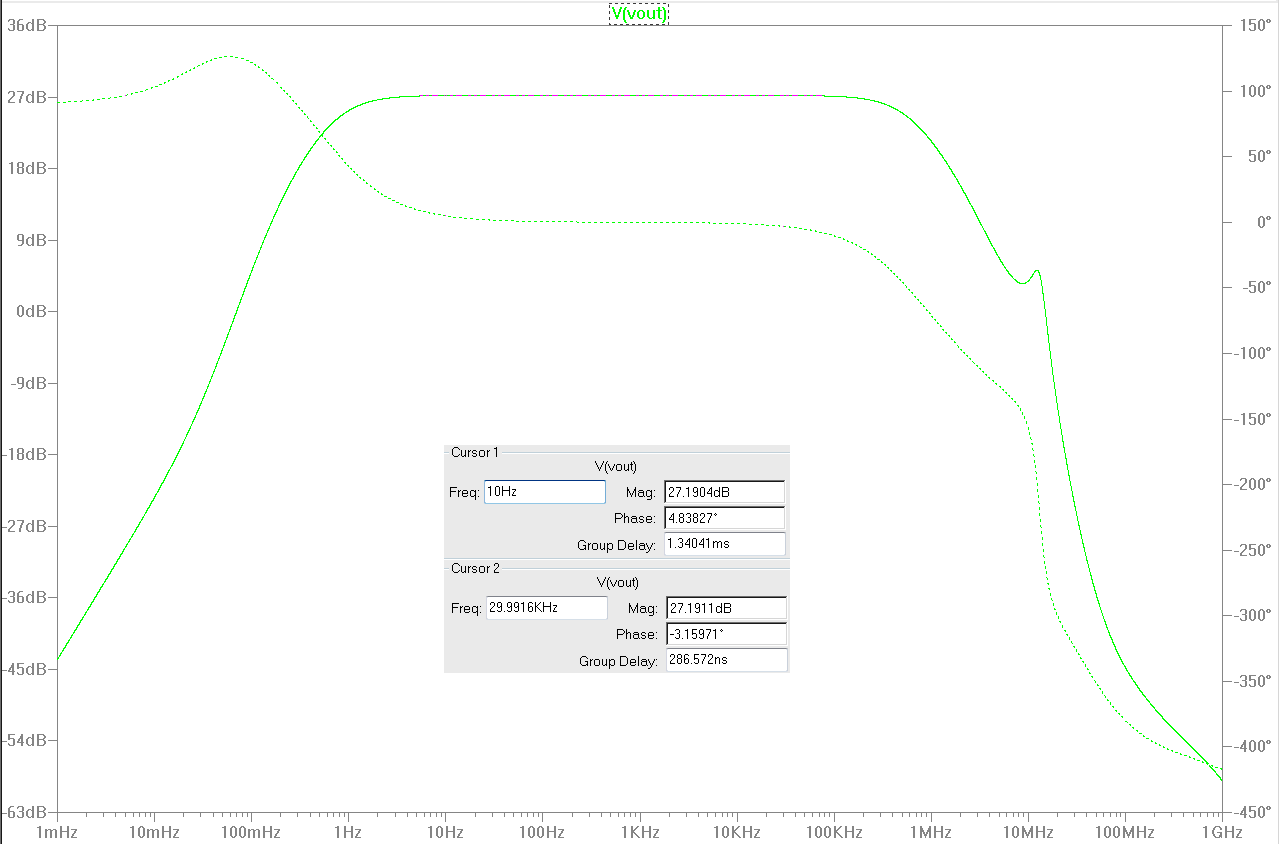
\includegraphics[width=\textwidth]{img/10hz-30khz.png}}
\caption{Respuesta en frecuencia.}
\label{resp_frec} 
\end{figure}

\bigskip
\subsubsection{Slew Rate}

Para esta simulación se utilizo el circuito de la Figura~\ref{cir_simul_slew_rate}, en el cual la entrada al amplificador es una señal escalón. Se simuló y se tomaron las tensiones en dos puntos, luego se aproxima el slew rate como la pendiente entre estos puntos. Como se ve en la Figura~\ref{simul_slew_rate} con los puntos elegidos se obtuvo un slew rate de $20.2~ \frac{\volt}{\usec}$.

\begin{figure}[H]
\centering
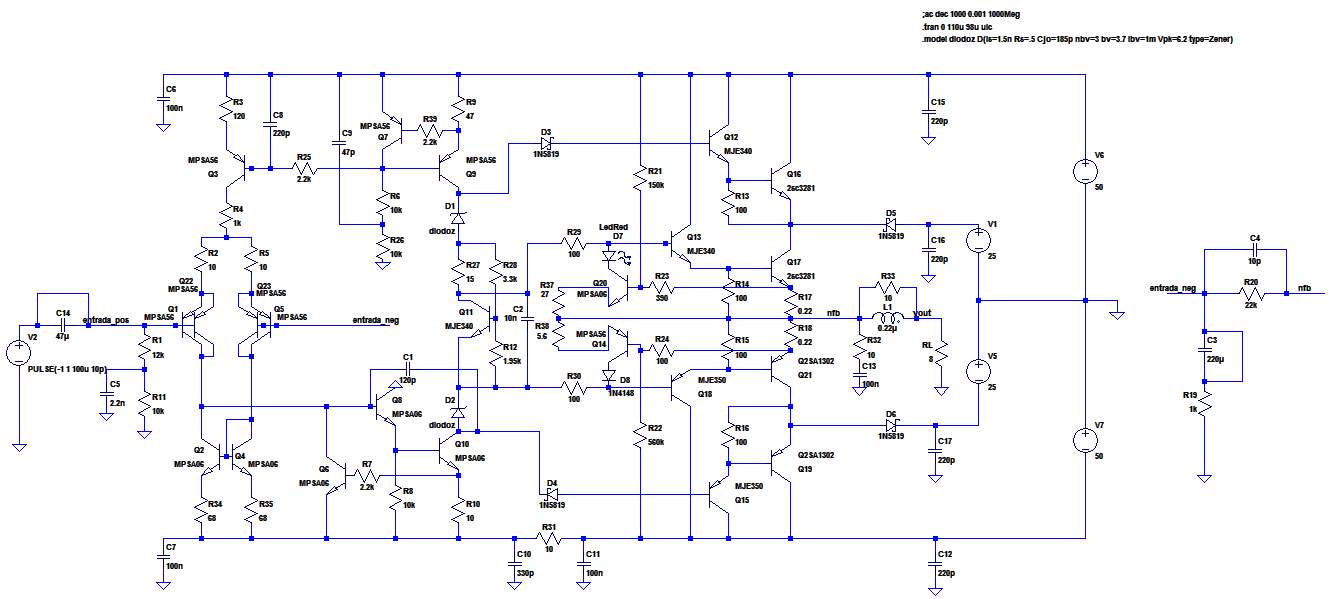
\includegraphics[width=1\textwidth]{img/slew_rate_cir.png}
\caption{Circuito utilizado para obtener slew rate.}
\label{cir_simul_slew_rate}
\end{figure}

\begin{figure}[H]
\centering
\centerline{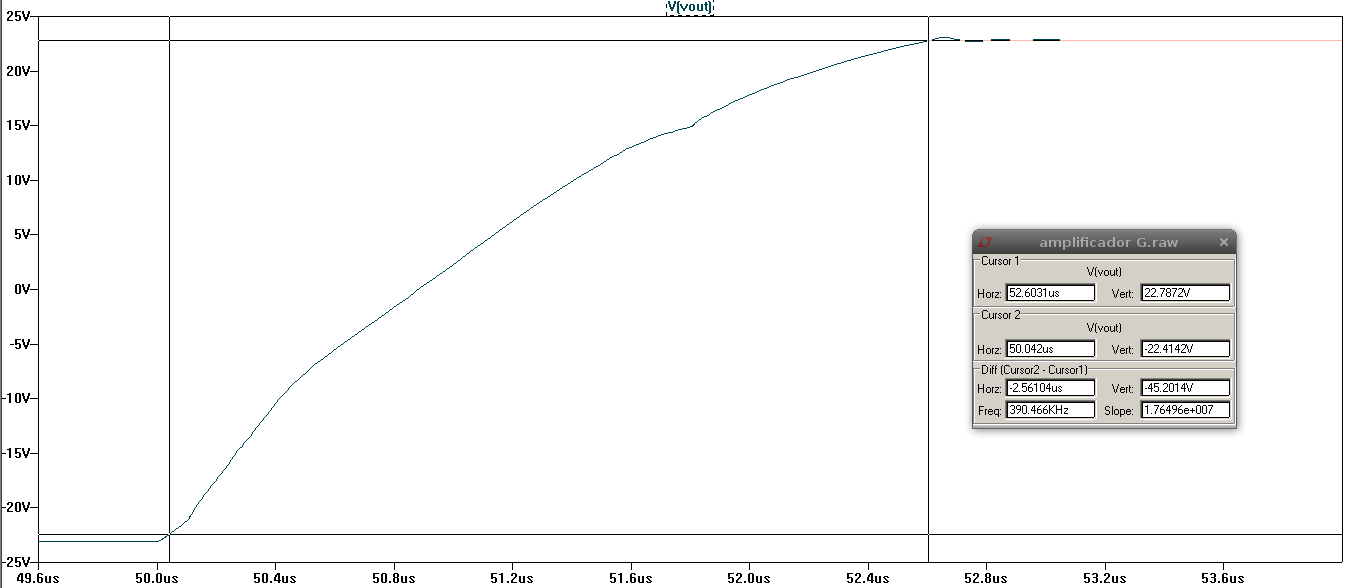
\includegraphics[width=1\textwidth]{img/slew_rate.png}}
\caption{Simulación del slew rate.}
\label{simul_slew_rate}
\end{figure}

\medskip
\subsubsection{Estabilidad}

Para obtener el margen de ganancia y fase del circuito se simuló la respuesta en frecuencia de la ganancia a lazo abierto(T), para eso se modificó la topologia del circuito como se ve en la Figura~\ref{cir_simul_estab}. Para obtener el margen de ganancia se determino la ganancia con un angulo de -180º, dando un margen de 11db. Por otro lado, el margen de fase resulto de 67º,siendo la diferencia entre la fase a 0db y -180º.
Los resultados de la simulación se observan en la Figura~\ref{simul_estab}.

\begin{figure}[H]
\centering
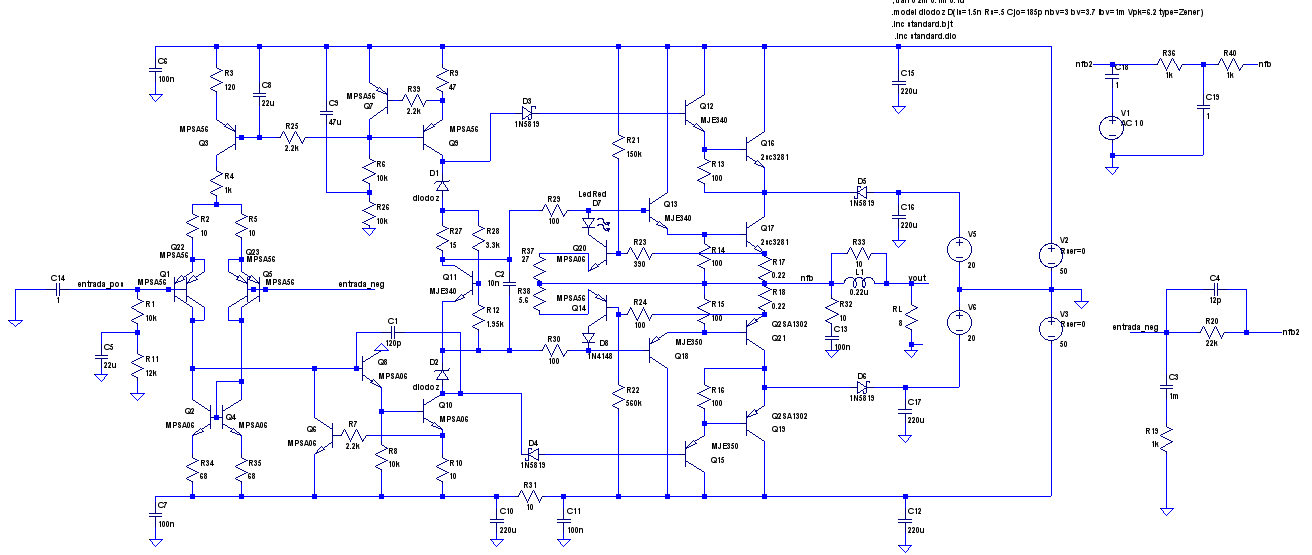
\includegraphics[width=1\textwidth]{img/margen_fase_ganancia_cir.png}
\caption{Circuito utilizado en análisis de estabilidad.}
\label{cir_simul_estab}
\end{figure}


\begin{figure}[H]
\centering
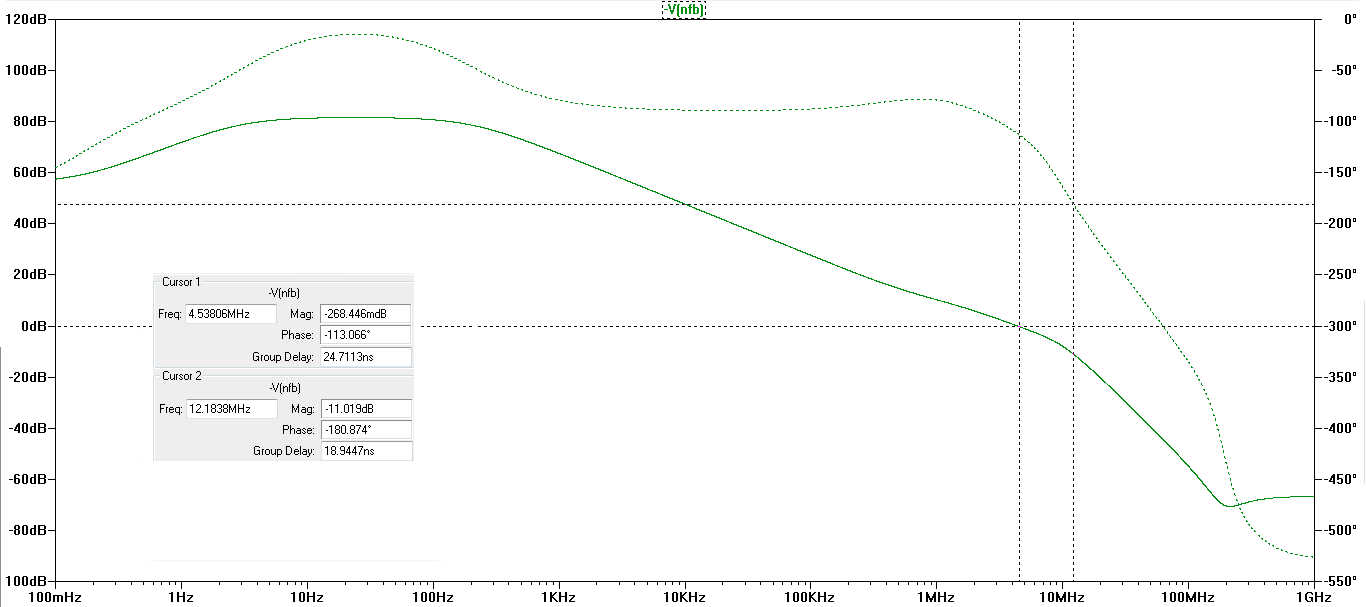
\includegraphics[width=1\textwidth]{img/margen_fase_ganancia.png}
\caption{Respuesta en frecuencia de T.}
\label{simul_estab}
\end{figure}



\medskip
